%!TEX encoding = UTF-8 Unicode

%!TEX root = ../compendium.tex


\Assignment{life}

\begin{Goals}
    \item Kunna använda matriser som en datastruktur.
    \item Kunna separera modell från vy med hjälp av \emph{Model-View}-uppdelning.
    \item Känna till grundläggande cellulära automata. % \eng{cellular automata}.
    % Följande rad är kanske inte aktuell, trådar tas upp i övningarna och hör inte riktigt hemma här då det är svårt att få in på ett smakligt sätt då Scala-kompilatorn och JVMen redan lyckas optimera koden så att den blir parallell.
    %\item Känna till trådar, en grundläggande metod för att köra flera metoder \emph{samtidigt}.
\end{Goals}


\begin{Preparations}
    \item Läs igenom laborationen.
    \item Bekanta dig med kodskelettet.
    \item Börja skriva konstruktorn för \code{ArrayMatrix2D} som handleds i uppgift 1a.
    % TODO: The following are just "fun" preparations, which will give the student more insight into the field but aren't
    %       actually required to complete the lab. They are optionals really.
    %\item Läs om Life på Wikipedia.
    %\item Läs om Cellulära automata på Wikipedia.
\end{Preparations}

\subsection{Bakgrund}

% Hur mycket bakgrund, vilken typ av bakgrund är lämplig/intressant/relevant?
Spelet Life (även kallat \emph{Conway's Game of Life} efter skaparen och matematikern John Horton Conway) simulerar en koloni av encelliga organismer som lever, förökar sig och dör på ett rutnät (även kallat bräde). Varje enskild cells överlevnad beror på dess omgivning, vilket kan beskrivas med några enkla regler. Detta är gemensamt för alla cellulära automater. Spelet går ut på att simulera flera generationer av någon uppsättning celler, en såkallad cellkoloni, startkonfiguration eller frö (eng. \textit{seed}). Många sådana cellkolonier kan i Life verka bete sig `levande' och spelet har därifrån fått sitt namn.\footnote{Detta är ett exempel på s.k. `emergence' och `self-organization'} Spelet har inga medvetna spelare (ett så kallat `zero-player game') och om reglerna följs så kommer slutresultatet fullständigt bero på startkonfigurationen.

\vspace{5mm}

I denna laboration ska vi implementera en datastruktur för brädet samt reglerna för Life.

I extrauppgifterna kommer det även finnas möjlighet att utforska två andra exempel på cellulära automater.

\vspace{5mm}

För mer om Game of Life, se Wikipedia:

\begin{itemize}[noitemsep,topsep=0pt]
    	\item Engelska: \url{https://en.wikipedia.org/wiki/Conway's_Game_of_Life}
    	\item Svenska: \url{https://sv.wikipedia.org/wiki/Game_of_Life}
\end{itemize}


\subsection{Reglerna i Life}
\label{subsec:life-rules}

Varje cells tillstånd i nästa generation bestäms av följande regler:
\begin{enumerate}
    \item Om en levande cell har två eller tre grannar så lever den vidare.
    \item Om en levande cell har mindre än två eller mer än tre grannar dör den (av underpopulation respektive överpopulation).
    \item Om cellen är död och har exakt tre grannar så föds den och dess tillstånd ändras till levande, annars fortsätter den vara död.
\end{enumerate}

Med grannar menas i Life de s.k. Moore-grannarna. Dessa är helt enkelt de närmsta omgivande cellerna vertikalt, horizontalt och diagonalt.

\begin{figure}[h]
  \begin{center}
    \includegraphics[width=0.5\textwidth]{../img/w12-lab/moore_neighborhood.png}
  \end{center}
  \caption{Moore-grannskapet består av nio celler: mittcellen samt de åtta omringande cellerna.\protect\footnotemark}
  \label{fig:threads:life:moore-neighborhood}
\end{figure}
\footnotetext{Källa: \url{https://commons.wikimedia.org/wiki/File:Moore_neighborhood_with_cardinal_directions.svg}}


\subsection{Beskrivning av Workspace}

I workspacet finner ni bl.a. paketen \code{models}, \code{rules} och \code{views}. I labben kommer ni främst ändra i \code{models}-paketet, men ni kommer även implementera reglerna för Life i \code{rules/LifeRule.scala}. Paketet \code{views} kommer med färdigimplementerad kod för två vyer \code{CellularConsoleView} samt \code{CellularGuiView}.

Utöver paketen finner ni i samma mapp några körbara Scala-filer som kan användas för att starta upp ett användargränssnitt som ritar upp brädet och låter användaren `spela' spelet. Den första av dessa filerna ni ska titta i och senare köra är \code{life.scala}.

Läs igenom de två filerna i \code{models}-paketet noga. Det är där ni kommer spendera den mesta av tiden.


\subsection{Obligatoriska uppgifter}
	% Förslag på hur de kan bygga upp programmet:
    % 1) skapa en main-klass som öppnar ett fönster som visar ett x gånger y stort fönster.
    % 2) [Kommer inte göras] skapa en klass Cell som har attributet levande eller död. Gör en metod där man kan ändra tillståndet på cellen.
    % 3) skapa en matris av celler som alla initieras som döda.
	% 4) koppla ihop modellen och vyn så att om man genom att klicka i vyn kan ändra cellens tillstånd. Testa att det fungerar. Gör så att vyn uppdateras efter cellerna i modellen när man klickar på "next generation".
	% 5) Studera traitet Rule i filen blahblah. Implementera reglerna (ge lite förklarande kodexempel för traitet Rule eller var det finns)
	% 6) Skriv metod(er) som räknar upp generationer.
	% 7) Testa nedanstående startfigurer (inkludera bilder på t ex en slider). Beter det sig som förväntat?


\Task Skapa en modell som kan visas i vyer som implementerar \code{CellularView2D}.

Spelbrädet består av en matris med $n$ rader och $m$ kolumner. ($n$ och $m$ brukar ibland modelleras som $\infty$, men vi kommer begränsa oss för enkelhetens skull).

Varje cell i matrisen kan vid varje tidpunkt (i varje generation) ha ett av två tillstånd: levande eller död. Dessa kommer vi för enkelhetens skull att representera som 1 eller 0, respektive. Detta för att göra det enklare att räkna ihop hur många levande grannar en cell har.

\Subtask Implementera konstruktorn i kompanjonsobjektet för \code{ArrayMatrix2D}.

För att skapa en matris ska vi använda oss av Scalas inbyggda datastruktur \code{Array}. Denna datastruktur har en användbar konstruktur \code{ofDim[T](n1: Int, n2: Int)} som vi ska använda för att skapa \emph{rows} stycken arrayer av storlek \emph{cols} inuti en annan array.

Ett exempel av resultatet från \code{Array.ofDim[Int](3, 3)} är följande ekvivalenta kod:

\begin{Code}
Array(
	Array(0,0,0),
	Array(0,0,0),
	Array(0,0,0)	
)
\end{Code}

% Här nedan ser vi en sådan array utskriven i en komma-separerad lista. Detta är ett vanligt och enkelt dataformat som kallas CSV.\footnote{Förkortningen CSV står för Comma Separated Values}

%\begin{Code}
%0,0,0
%0,0,0
%0,0,0
%\end{Code}

\Subtask Implementera de övriga metoderna i \code{ArrayMatrix2D}. Läs igenom kommentarerna för de oimplementerade metoderna i traitet \code{Matrix2D} för kommentarer om vad som ska göras.


\Subtask Testa implementationen. Ta gärna hjälp av metoden \code{randomize} som finns på alla objekt som ärver traitet \code{Matrix2D}. Med den kan man enkelt slumpa fram nya tillstånd på brädet på följande vis:

\begin{Code}
// Slumpar varje cell i matrisen 'matrix' till antingen 0 eller 1
matrix.randomize(2)
\end{Code}

För att nu kontrollera att allt har blivit rätt kan vi visa upp matrisen i terminalen med hjälp av \code{CellularConsoleView}. Ett exempel på detta finns i \code{life_console.scala}.

\begin{Code}
// Skriver ut brädet i konsolen
CellularConsoleView.display(matrix)
\end{Code}

Men detta testar inte för alla möjliga fel, så för säkerhets skull kan vi även testa att placera ut en s.k. glider i brädet med hjälp av metoden \code{place} som finns implementerad i det ärvda traitet \code{Matrix2D}.

\begin{Code}
// Placerar ut en glider med sitt övre vänstra hörn i punkten
// (3, 1), d.v.s. på rad 4 och kolumn 2 (då vi noll-indexerar)
matrix.place(entities.glider, 3, 1)
\end{Code}

\begin{figure}[h]
  \begin{center}
    % Reflectbox here since glider in entities package is a reflection of the image.
    \reflectbox{\includegraphics[width=0.3\textwidth]{../img/w12-lab/glider.png}}
  \end{center}
  \caption{En så kallad \textit{glider}. Vanligt förekommande varelse i Life.}
  \label{fig:threads:life:glider}
\end{figure}

Testa nu att rita ut brädet igen (utan \code{randomize} den här gången) för att se till att glidern hamnade rätt både med avseende på orientering och position. Den ska vara roterad precis som i figur \ref{fig:threads:life:glider}.


\Task Implementera Life-regeln med hjälp av traitet \code{Rule}.

Nu har vi vår datastruktur för brädet på plats, så det är dags att faktiskt implementera reglerna för Life. För att göra detta ska vi implementera objektet \code{LifeRule} som ärver traitet \code{Rule} vilket är ett interface som cellulära automaters regler kan implementera. Men först ska vi implementera några hjälpsamma funktioner, så att vår kod i \code{LifeRule} senare blir mer lättläst.

\Subtask Implementera \code{mooreNeighborsPositions} samt \code{mooreNeighborsStates} i \code{Matrix2D}.

Då Life-regeln förlitar sig på Moore-grannskapet som tidigare nämnts så behöver vi ett smidigt sätt att få ut grannarna för en viss cell. Detta är vad funktionerna \code{mooreNeighborsPositions} samt \code{mooreNeighborsStates} ska göra.

När \code{mooreNeighborsStates} implementeras är det viktigt att ta hänsyn till om grannarna faktiskt finns (då vårt bräde är av begränsad storlek).
För detta bör man använda \code{isWithinMatrix}-metoden som tidigare implementerades i \code{ArrayMatrix2D}.

Börja med att implementera \code{mooreNeighborsPositions} och använd sedan den för att implementera \code{mooreNeighborsStates}.

\Subtask Implementera \code{apply} i ett nytt objekt \code{LifeRule} som implementerar \code{Rule}.

Nedan finns specifikationen för traitet \code{Rule}. Den innehåller endast en metod \code{apply} vars uppgift är att ta ett bräde samt en position på brädet och returnera vad denna position ska innehålla för värde i nästa generation.

\begin{ScalaSpec}{Rule}
// apply tar en matris samt en position i matrisen (row, col)
// och applicerar regeln på den positionen
def apply(m: ArrayMatrix2D, row: Int, col: Int): Int
\end{ScalaSpec}

Reglerna för Life finner ni ovan i avsnitt \ref{subsec:life-rules}.

\Subtask Testa implementationen.

För att nu i praktiken applicera vår regel på brädet ska vi använda oss av metoden \code{applyRule} som finns i \code{ArrayMatrix2D}.

Om man har problem med att sin regel inte beter sig som förväntat kan man felsöka genom att returnera antalet grannar istället för cellens levande/död-tillstånd. Efter att ha applicerat hela s.k. \code{NeighborsRule} kan man visa upp resultatet med \code{CellularConsoleView} för att se om programmet räknar grannar korrekt.


\Task Skapa en ny modell som ''wrappar'' i kanterna.

Just nu har vi ett udda beteende i modellen, nämligen att alla celler utanför brädet i praktiken räknas som döda. För att få ett lite mer intressant beteende vill vi nu göra så att om exempelvis en glider åker in i höger vägg ska den komma ut ur vänster vägg. Detta kan göras med några små modifikationer till \code{ArrayMatrix2D}.

\Subtask Ändra metoden \code{isWithinMatrix} så att alla positioner är giltiga.

Då funktionen \code{mooreNeighborsStates} i \code{Matrix2D} använder sig av funktionen \code{isWithinMatrix} för att avgöra om celler är inom brädet måste vi se till att \code{isWithinMatrix} inte hindrar grann-funktionen från att hämta celler ''utanför'' brädet. Detta kan vi enkelt göra genom att kommentera ut hela den tidigare koden och istället alltid returnera \code{true}. Om vi nu försöker köra programmet kommer vi få \code{ArrayIndexOutOfBoundsException} eftersom vi ännu inte gjort så att hämtningar eller tilldelningar ''utanför'' brädet wrappar, vilket vi nu ska göra.

\Subtask Ändra metoderna \code{get} samt \code{set} så att hämtningar respektive tilldelningar utanför brädet wrappar.

För att åstadkomma wrappning måste vi göra så att alla hämtningar och tilldelningar utanför brädet ''går runt''. Detta kan enklast göras med hjälp av modulo-operatorn.

\begin{Code}
val wrapped_row = row % rows
\end{Code}

Men denna lösning tar inte hänsyn till negativa tal, vilket kan uppkomma när man t.ex. försöker hämta grannarna för cellen i det övre vänstra hörnet på brädet, d.v.s. position (0, 0). För att enkelt lösa detta kan man förskjuta hela \code{row} med \code{rows} så att man istället får följande:
		
\begin{Code}
val wrapped_row = (rows + row) % rows
\end{Code}

Vi kan använda oss av denna kunskap för att i metoderna \code{get} samt \code{set} se till att operationerna wrappar. Testa sedan din implementation genom att låta en glider glida in i en vägg.


\subsection{Frivilliga extrauppgifter}

Inom cellulära automata finns det många intressanta ting att utforska. Nedan finns några extrauppgifter som nyfikna och intresserade läsare uppmanas implementera då resultaten kan vara djupt tillfredställande. De kan göras i valfri ordning.


\Task Implementera spara och ladda.

När man leker runt med cellulära automater vill man ofta spara sina bräden så att man senare enkelt kan ladda in dem igen. För att göra detta ska vi i denna extrauppgift definiera ett dataformat som ska innehålla all data som behövs för att återskapa vår \code{ArrayMatrix2D}.

\Subtask Spara brädets tillstånd.

Tillståndet ska sparas till ett format som både är lätt att spara/exportera och ladda/importera. Det vi behöver spara är följande:

\begin{itemize}
	\item Brädets storlek, d.v.s. antalet rader och kolumner
	\item Hur många olika värden en cell på brädet kan anta
	\item Matrisen i sig, d.v.s. alla cellers värden
\end{itemize}
        	
Det är metoden \code{ArrayMatrix2D.toFileFormat} som ska implementeras.
        
Vi föreslår att ni börjar filen med en rad innehållande de två värdena i punkt ett, samt värdet i punkt två. Separera dem med mellanslag, komma, eller en emoji (på egen risk). Därefter är det lämpligt att skriva ut matrisen rad för rad där varje cell skrivs ut som en etta eller nolla. Man kan göra detta utan separator för bräden där celler bara antar värden i intervallet 0-9, men det fungerar inte längre om en cell kan anta andra värden (såsom i uppgiften med cykliska cellulära automater nedan) då man inte längre kan lita på att en cell motsvaras av en enda siffra. För att lösa denna begränsning kan man separera sina värden med något tecken precis som för första raden.

Testa att spara genom att gå in i menyn i användargränssnittet och välja ''Save...''. Öppna den sparade filen med en texteditor för att verifiera att innehållet ser korrekt ut.

\Subtask Ladda in det sparade tillståndet.

Implementera metoden \code{ArrayMatrix2D.fromFileFormat} för att läsa in det sparade tillståndet.

Testa sedan att ladda genom att gå in i menyn i användargränssnittet och välja ''Load...''. Brädet ska nu se ut precis som det gjorde när det sparades.

\Task Implementera andra regler för cellulära automata.

Det finns massor med regler för cellulära automata med sina egna intressanta beteenden och tillstånd.
Gör den eller de du tycker verkar mest intressant!

Fler regler finns här: \url{https://en.wikipedia.org/wiki/Category:Cellular_automaton_rules}

Nedan följer några roliga exempel som valts ut och anses lämpliga.

\Subtask Implementera regeln för cykliska cellulära automater.

Denna typ av automata kallas cyklisk just för att det finns $N$ möjliga tillstånd och när tillståndet $N-1$ nås så är ''nästa'' tillstånd $0$.
Detta beteende kan beskrivas med modulo-operatorn: $T_{nästa} = (T_{nuvarande} + 1)\ \%\ N$

Regeln är att om en granne till den aktuella cellen har tillståndet exakt ett över cellens tillstånd så får cellen sin grannes tillstånd. Det vill säga om en granne har tillståndet $T_{nästa}$ så får även cellen i mitten det värdet.

För att få intressant beteende brukar man initialisera hela brädet så att varje cell får ett slumpvalt tillstånd.

En bra förberedelse för att implementera denna cellulära automat är att läsa Wikipedia-artikeln: \url{https://en.wikipedia.org/wiki/Cyclic_cellular_automaton}

    \Subtask{Implementera regeln för Wireworld.}

Wireworld skiljer sig från andra cellulära automata då man i Wireworld designar `kretsar' inte helt olika de som finns i moderna datorer.
På grund av detta är majoriteten av celler vanligtvis fast i ett dött tillstånd (isolatorer).

I Wireworld kan man skapa komponenter såsom dioder och transistorer. Med dessa kan man bygga logiska grindar och därmed hela datorer (som dock blir väldigt långsamma i jämförelse med datorerna de körs på).

En bra förberedelse för att implementera Wireworld är att läsa Wikipedia-artikeln: \url{https://en.wikipedia.org/wiki/Wireworld}

\begin{figure}[h]
    \begin{center}
        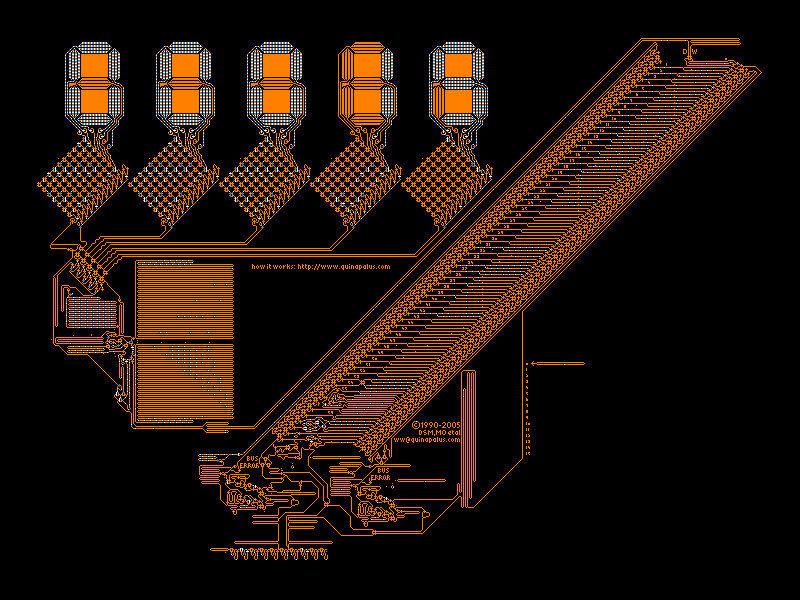
\includegraphics[width=0.8\textwidth]{../img/w12-lab/wireworld_computer.png}
    \end{center}
    \caption{En enkel dator implementerad i Wireworld.\protect\footnotemark}
    \label{fig:threads:life:wireworld-computer}
\end{figure}
\footnotetext{Källa: \url{http://www.quinapalus.com/wi-index.html}}


\subsection{Extra läsning}

\subsubsection{Intressanta mönster i Life}

\begin{itemize}[noitemsep,topsep=0pt]
    \item \url{https://en.wikipedia.org/wiki/Spacefiller}
    \item \url{https://en.wikipedia.org/wiki/Spaceship_(cellular_automaton)}
\end{itemize}

\subsubsection{Intressanta automater}

\begin{itemize}[noitemsep,topsep=0pt]
	\item \url{https://en.wikipedia.org/wiki/Codd's_cellular_automaton}
	\item \url{https://en.wikipedia.org/wiki/Von_Neumann_universal_constructor}
\end{itemize}

\subsubsection{Intressanta resurser}

\begin{itemize}[noitemsep,topsep=0pt]
    \item Eric Weisstein's Treasure Trove of the Life Cellular Automaton: \url{http://www.ericweisstein.com/encyclopedias/life/topics/}
\end{itemize}



% Kanske för nästa år
%\Task{Alternativ vy: Kör programmet i webbläsaren med Scala.js}


% Detta kan kräva speciell IDE (android-studio) och eventuellt en Android-emulator som inte kan köras på skolans datorer.
%\Task{Alternativ vy: Kör programmet på Android}


% Detta kommer antagligen inte ske då det lägger till signifikant komplexitet
% En bättre extrauppgift är att representera brädet som ett quadtree då det leder en in på Hashlife
%\Task{Implementera brädet som en sparse-matris}

%I den tidigare lösningen har vi allokerat en hel matris där bara en del av brädet vanligtvis är levande, en sådan matris kallas för en sparse matris (en matris där majoriteten av värdena är 0).
%    \Subtask{???}


%\Task{Implementera den supersnabba Hashlife}
%    Detta är en utmaning som kräver en viss kunskap om algoritmer och hashning som läsare av denna labben inte ännu förväntas inneha.
%    Den verkligt intresserade läsaren kan dock se denna uppgift som ett långtids-läromål och återkomma till uppgiften senare i sin utbildning när
%    hen känner sig redo.
%
%    En utförlig beskrivning om hashlife och quadtrees finnes på Wikipedia:
%    \begin{enumerate}
%        \item https://en.wikipedia.org/wiki/Hashlife
%        \item https://en.wikipedia.org/wiki/Quadtree
%    \end{enumerate}
%
%    \Subtask{Implementera QuadtreeMatrix2D}
%        Hashlife använder sig inte av en matris-representation för brädet utan använder sig istället av en datastruktur som heter Quadtrees.
%        Dessa fungerar som vanliga träd fast varje nod kan antingen ha exakt 4 brancher eller vara ett löv. Varje branchning delar upp en kvadrat
%        i 4 mindre kvadrater och varje löv representerar värdet för en kvadrat.
%
%        Quadtrees möjliggör att man kan beräkna tomma områden på brädet på konstant tid då man vet att ett helt område kommer förbli opåverkat utan
%        att behöva titta igenom varje cell.
%
%        \begin{figure}[h]
%            \begin{center}
%                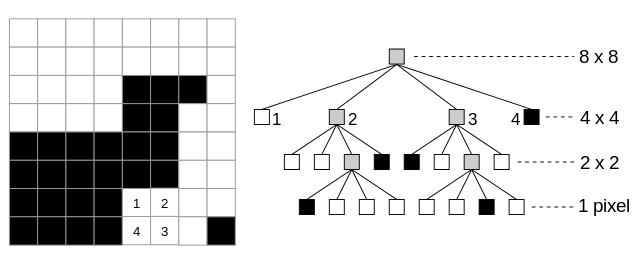
\includegraphics[width=0.7\textwidth]{../img/w12-lab/quadtree_bitmap.png}
%            \end{center}
%            \caption{Ett exempel på hur ett Quadtree använts för att representera en bitmap likt den som återfinns i Life}
%            % Källa: Wikipedia (https://commons.wikimedia.org/wiki/File:Quad_tree_bitmap.svg)
%        \end{figure}
%
%    \Subtask{Implementera hashlife}
%
%        Här kan vi inte handleda er, då det anses vara allt för långt utanför kursmålen. Men för den ambitiösa studenten refererar vi glatt till Wikipedia och önskar er lycka till!
